\section{Dynamische Race Detection durch Locksets}

In dieser Sektion wird Dynamische Race Detection durch Locksets betrachtet und anhand von Eraser nähergebracht. Auf einem hohen Level überprüft Eraser, ob geteilter Speicherzugriff einem konsistentem Lock Mechanismus geschützt ist. Auf Locks wird in Kapitel \hyperref[sec:loesen]{5} weiter eingegangen \cite[vgl.][392]{savage_eraser_nodate}.

\subsection*{Eraser}

\subsubsection*{Lockset Refinement}

Erasers Lock Mechanismus ist, ob jeder Zugriff auf eine geteilte Variable durch ein Schloss gesichert ist. Dieser Mechanismus wird überprüft, indem Eraser alle Zugriffe auf den Speichert überwacht. Das Problem dabei ist, dass Eraser nicht weiß, welches Lock für welche Variable ist \cite[vgl.][396]{savage_eraser_nodate}. 

Um dies herauszufinden, benutzt Eraser Lockset Refinement. Für jede geteilte Variable \texttt{v} hat Eraser ein Set \texttt{C(v)} an möglichen Locks für \texttt{v}. Bei jedem Zugriff auf \texttt{v} von einem Thread wird die Schnittmenge zwischen die aktuellen Locks \texttt{locks\_held} und \texttt{C(v)} gebildet und zurück in \texttt{C(v)} geschrieben. Wenn \texttt{C(v)} nun leer ist liegt ein Data Race vor. Dargestellt ist dieser Mechanismus in \ref{tab:locksetRefinment} \cite[vgl.][396-397]{savage_eraser_nodate}. 

%\begin{comment}
\begin{table}[h]
    \myfloatalign
    \begin{tabularx}{\textwidth}{XXX} \toprule
        \tableheadline{Program} & \tableheadline{locks\_held}
        & \tableheadline{C(v)} \\ 
        \midrule
        lock(mu1); & \{ \} &  \{ mu1, mu2 \} \\
        v := v + 1; & \{ mu1 \} & \{ mu1, mu2 \} \\
        unlock(mu1); & \{ \} & \{ mu1 \} \\
        \midrule
        lock(mu2); & \{ \} & \{ mu1 \} \\
        v := v + 1; & \{ mu2 \} & \{ mu1 \} \\
        unlock(mu1); & \{ \} & \{ \} \\
        \bottomrule
    \end{tabularx}
    \caption[Lockset Refinment]{Lockset Refinment \cite[397]{savage_eraser_nodate}}
    \label{tab:locksetRefinment}
\end{table}
%\end{comment}

\subsubsection*{Verbesserungen von Lockset Refinement}

Der Lock Mechanismus ist jedoch zu restriktiv. Um diesen zu Verbessern nimmt Eraser drei Szenarien aus dem Lock Mechanismus, die ein Data Race verursachen würden, aber keines sind. Diese drei Szenarien sind: Die Initialisierung einer geteilten Variable, Read-Shared Data, also Varaiblen die nach einmaligen initialisieren nur noch gelesen werden, und Read-Write Locks, welches Variablen sind, auf die nur ein Thread mit Schreiboperationen zugreift \cite[vgl.][396-397]{savage_eraser_nodate}. 

In \ref{fig:eraserState} dargestellt sind die Zustände, welche eine geteilte Variable bei der verbesserten Version des Lockset Refinements haben kann. Bei der Initialisierung wird der Zustand der Variable auf den \texttt{Virgin} Zustand gesetzt. Sobald ein Thread auf die Variable zugreift, ändert sich der Zustand zu \texttt{Exclusive} und bleibt solange in diesem Zustand bis ein neuer Thread auf die Variable zugreift. Wenn eine Lese Operation von dem neuen Thread ausgeht, ist der neue Zustand \texttt{Shared}. Wird von dem neuen Thread jedoch eine Schreib Operation ausgeführt, geht die Variable in den \texttt{Shared-Modified} Zustand. Um die oben genannten Fälle zu lösen, wird ein Data Race nur im \texttt{Shared-Modified} Zustand berichtet \cite[vgl.][397-399]{savage_eraser_nodate}.   

%\begin{comment}
\begin{figure}[ht]
    \centering
    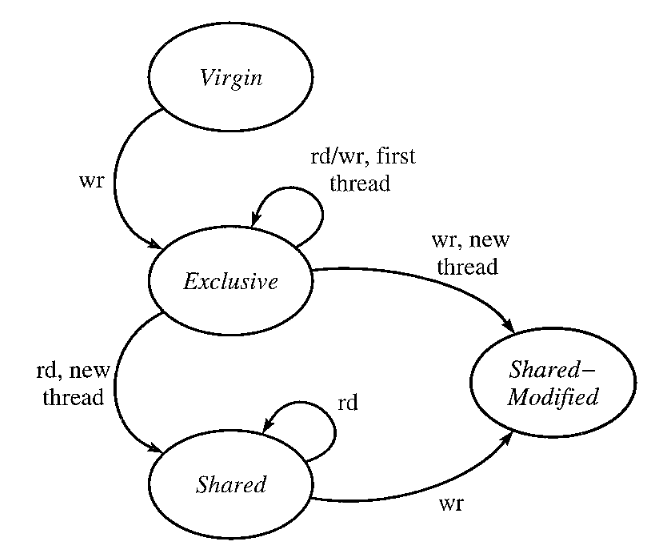
\includegraphics[width=0.5\textwidth]{gfx/eraser_state.png}
    \caption{Eraser States \cite[389]{savage_eraser_nodate}}
    \label{fig:eraserState}
\end{figure}
%\end{comment}

\subsection*{Leistung}

\textcite[vgl.][400]{savage_eraser_nodate} beschreiben, dass Leistung nicht das primäre Ziel bei Eraser war und dementsprechend noch viele Stellen Verbesserungsmöglichkeiten. 

Programme, auf die Eraser angewendet wird, sind um einen Faktor von 10 bis 30 langsamer als ohne. Zudem kann Thread Scheduling einen Einfluss auf das Ergebnis von Eraser haben kann \cite[vgl.][400]{savage_eraser_nodate}.   

%\subsection{Auswertung}

